
\chapter[Dạng bài: Phương trình sóng cơ]{Dạng bài: Phương trình sóng cơ}
\section{Lý thuyết}
\subsection{Phương trình sóng}
\begin{center}
	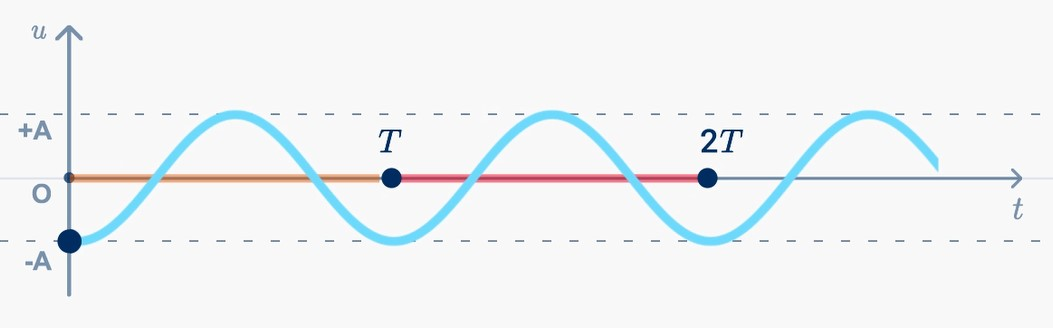
\includegraphics[scale=0.6]{../figs/VN12-PH-10-A-006-1-V2-1.jpg}
\end{center}
\subsubsection{Phương trình sóng tại nguồn}
Xét một sóng hình $\sin$ lan truyền trong một môi trường, sóng này phát ra từ một nguồn điểm O. Giả sử phương trình dao động tại nguồn O có dạng:
\begin{equation*}
	u_{\text{O}} = A\cos (\omega t + \varphi_0),
\end{equation*}

với $u_\text O$ là li độ tại O tại thời điểm $t$.

\subsubsection{Phương trình sóng tại một điểm nằm trên phương truyền sóng}	
Phương trình sóng tại điểm M cách nguồn một đoạn $d$:
\begin{itemize}
	\item Nếu sóng truyền theo chiều dương:
	
	\begin{equation*}
		u_{\text{M}} = A\cos \left(\omega t + \varphi_0 - \dfrac{2\pi d}{\lambda}\right).
	\end{equation*}
	
	\item Nếu sóng truyền theo chiều âm:
	
	\begin{equation*}
		u_{\text{M}} = A\cos \left(\omega t + \varphi_0 + \dfrac{2\pi d}{\lambda}\right).
	\end{equation*}
	
\end{itemize}

\luuy{Phương trình sóng là một hàm vừa tuần hoàn theo thời gian, vừa tuần hoàn theo không gian.}
\subsection{Độ lệch pha}
Xét 2 điểm M, N cách nguồn O các đoạn $x_1$, $x_2$ trên cùng phương truyền sóng.
\begin{center}
	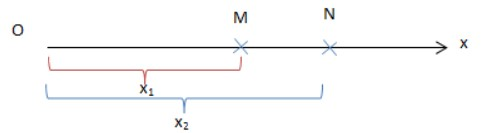
\includegraphics[scale=0.9]{../figs/VN12-PH-10-A-006-1-V2-2.jpg}
\end{center}

Độ lệch pha giữa hai điểm M, N cách nguồn khoảng $d_{\text{M}}$, $d_{\text{N}}$ là

\begin{equation*}
	\Delta \varphi =\dfrac{2\pi d}{\lambda} = \dfrac{2\pi (d_{\text{N}}-d_{\text{M}})}{\lambda}.
\end{equation*}
\begin{itemize}
	\item Nếu sóng truyền từ M đến N thì $\Delta \varphi < 0$.
	
	\item Nếu sóng truyền từ N đến M thì $\Delta \varphi > 0$.
	
	\item Nếu M, N dao động cùng pha thì $\Delta \varphi =2k \pi$.
	\item Nếu M, N dao động ngược pha thì $\Delta \varphi = (2k+1) \pi$.
	\item Nếu M, N dao động vuông pha thì $\Delta \varphi = (2k +1) \dfrac{\pi}{2}$.
\end{itemize}
\section{Mục tiêu bài học - Ví dụ minh họa}
\begin{dang}{Giải thích được các đại lượng có trong phương trình sóng cơ}
	\viduii{2}{Một sóng ngang truyền theo chiều dương trục O$x$ có phương trình sóng là\\ $u=6\cos(4\pi t - 0,02 \pi x)$; trong đó $x$ tính bằng cm, $t$ tính bằng s. Sóng này có bước sóng:
		\begin{mcq}(4)
			\item 150 cm.
			\item 50 cm.
			\item 100 cm.
			\item 200 cm.
		\end{mcq}
	}
	{
		\begin{center}
			\textbf{Hướng dẫn giải}
		\end{center}
		
		Trong phương trình sóng trên thì $\dfrac{2\pi x}{\lambda} = 0,02 \pi x$. Suy ra:
		$$\dfrac{2\pi}{\lambda}=0,02 \pi \Rightarrow \lambda=100\ \text{cm}$$
		
		
		\textbf{Đáp án: C}.
	}
	
	\viduii{2}
	{
		Sóng cơ có tần số $\SI{80}{Hz}$ lan truyền trong một môi trường với vận tốc $\SI{4}{\meter/\second}$. Dao động của các phần tử vật chất tại hai điểm trên một phương truyền sóng cách nguồn sóng những đoạn lần lượt $\SI{31}{cm}$ và $\SI{33.5}{cm}$, lệch pha nhau góc
		\begin{mcq}(4)
			\item $\xsi{0.5\pi}{\radian}$.
			\item $\xsi{\pi}{\radian}$.
			\item $\xsi{1,5\pi}{\radian}$.
			\item $\xsi{2\pi}{\radian}$.
		\end{mcq}
	}{
		\begin{center}
			\textbf{Hướng dẫn giải}
		\end{center}
		
		Độ lệch pha của các phần tử tại hai điểm này là:
		$$\Delta \varphi =\frac{2\pi \Delta x}{\lambda }=\frac{2\pi f (x_1-x_2)}{v}=\frac{2\pi \cdot\SI{80}{Hz}\cdot(\SI{0.335}{\meter}-\SI{0.31}{\meter})}{\SI{4}{\meter/\second}}=\xsi{\pi}{\radian}.$$
		
		\textbf{Đáp án: B.}
	}
	
\end{dang}
\begin{dang}{Xây dựng được phương trình sóng cơ}
	\viduii{2}{Một nguồn dao động đặt tại điểm O trên mặt chất lỏng nằm ngang phát ra dao động điều hòa theo phương thẳng đứng với phương trình $u_\text O = A \cos \omega t$. Sóng do nguồn dao động này tạo ra truyền trên mặt chất lỏng có bước sóng $\lambda$ tới điểm M cách O một khoảng $x$. Coi biên độ sóng và vận tốc sóng không đổi khi truyền. Phương trình dao động tại M là
		\begin{mcq}(2)
			\item $u_\text M = A \cos \omega t$.
			\item $u_\text M = A \cos \left(\omega t-\dfrac{\pi x}{\lambda}\right)$.
			\item $u_\text M = A \cos \left(\omega t+\dfrac{\pi x}{\lambda}\right)$.
			\item $u_\text M = A \cos \left(\omega t-\dfrac{2\pi x}{\lambda}\right)$.
		\end{mcq}
	}
	{
		\begin{center}
			\textbf{Hướng dẫn giải}
		\end{center}
		
		Phương trình dao động tại M cách O một khoảng $x$ theo phương truyền sóng là $$u_\text M = A \cos \left(\omega t-\dfrac{2\pi x}{\lambda}\right)$$
		
		\textbf{Đáp án: D}.
	}
	
	\viduii{3}
	{
		Ở một mặt nước (đủ rộng), tại điểm O có một nguồn sóng dao động theo phương thẳng đứng với phương trình ${u}_{\text{O}}=6\cos 20\pi t$ ($u$ tính bằng cm, $t$ tính bằng s). Tốc độ truyền sóng trên mặt nước là $\SI{40}{cm/\second}$, coi biên độ sóng không đổi khi sóng truyền đi. Phương trình dao động của phần tử nước tại điểm M (ở mặt nước), cách O một khoảng $\SI{50}{cm}$ là
		\begin{mcq}(2)
			\item ${{u}_{\text{M}}}=6\cos\left( 20\pi t-\pi\right)\,\SI{}{cm}$.
			\item ${{u}_{\text{M}}}=6\cos\left( 20\pi t-\dfrac{\pi }{4} \right)\,\SI{}{cm}$.
			\item ${{u}_{\text{M}}}=4\cos\left( 20\pi t-\pi \right)\,\SI{}{cm}$.
			\item ${{u}_{\text{M}}}=4\cos\left( 20\pi t-\dfrac{\pi }{4} \right)\,\SI{}{cm}$.
		\end{mcq}
	}{
		\begin{center}
			\textbf{Hướng dẫn giải}
		\end{center}
		
		Bước sóng của sóng này là
		$$\lambda=\dfrac{v}{f}=\dfrac{v}{\dfrac{\omega}{2\pi }}=\dfrac{2\pi v}{\omega}=\dfrac{2\pi \cdot40\textrm{ cm/s}}{20\pi\,\SI{}{\radian/\second}}=\SI{4}{\centi\meter}.$$ 
		
		Độ lệch pha của sóng tại O so với sóng tại M là
		$$\Delta \varphi =\dfrac{2\pi \Delta x}{\lambda }=\dfrac{2\pi \cdot\SI{50}{\centi\meter}}{\SI{4}{\centi\meter}}=25\pi\,\SI{}{\radian}=\pi\,\SI{}{\radian}.$$
		
		Sóng truyền từ O đến M nên phương trình dao động sóng tại M là
		$${{u}_{\text{M}}}=6\cos \left( 20\pi t-\pi \right)\SI{}{\centi\meter}.$$
		
		\textbf{Đáp án: A.}
	}
	
\end{dang}
\begin{dang}{Sử dụng được phương trình sóng cơ\\ để xác định giá trị tức thời của li độ}
	\viduii{2}{Một sóng cơ lan truyền trên một sợi dây rất dài có phương trình $u=6 \cos (4\pi t - 0,02 \pi x)$; trong đó $u$ và $x$ có đơn vị là cm và $t$ có đơn vị là s. Hãy xác định li độ dao động của một điểm trên dây có tọa độ $x=25\ \text{cm}$ tại thời điểm $t=4\ \text s$.
		
		\begin{mcq}(4)
			\item 0 cm.
			\item 6 cm.
			\item 3 cm.
			\item -6 cm.
		\end{mcq}
	}
	{
		\begin{center}
			\textbf{Hướng dẫn giải}
		\end{center}
		
		Thay $x=25\ \text{cm}$ và $t=4\ \text s$ vào phương trình $u=6 \cos (4\pi t - 0,02 \pi x)$, ta được $u=0\ \text{cm}$.
		
		
		\textbf{Đáp án: A}.
	}
	
	\viduii{3}
	{
		Sóng truyền từ O đến M với vận tốc $v=40\ \text{cm/s}$, phương trình sóng tại O là\\ $u_\text O = 4 \sin \frac{\pi t}{2}\ \text{cm}$. Biết vào thời điểm $t$ thì li độ của phần tử M là 3 cm và đang chuyển động theo chiều dương. Lúc $t+6\ \text s$ thì li độ của M là
		
		\begin{mcq}(4)
			\item $-3$ cm.
			\item $-2$ cm.
			\item 2 cm.
			\item 3 cm.
		\end{mcq}
	}{
		\begin{center}
			\textbf{Hướng dẫn giải}
		\end{center}
		
		Ta có $T=\dfrac{2\pi}{\omega} = 4\ \text s$.
		
		Suy ra: $t+6 = t + T + \dfrac{T}{2}$. 
		
		Vào thời điểm $t$ thì li độ của phần tử M là 3 cm và đang chuyển động theo chiều dương, vậy vào thời điểm $t+6$ thì li độ của phần tử M là $-3$ cm và đang chuyển động theo chiều âm.
		
		\textbf{Đáp án: A.}
		
	}
	
\end{dang}
\begin{dang}{Sử dụng được phương trình sóng cơ\\ để xác định tốc độ truyền sóng}
	\viduii{3}{Một nguồn phát sóng cơ dao động theo phương trình $u = 4 \cos \left(4\pi t -\dfrac{\pi}{4}\right)\ \text{cm}$. Biết dao động tại hai điểm gần nhau nhất trên cùng một phương truyền sóng cách nhau 0,5 m có độ lệch pha $\dfrac{\pi}{3}$. Tốc độ truyền của sóng đó là
		
		\begin{mcq}(4)
			\item 1,0 m/s.
			\item 2,0 m/s.
			\item 1,5 m/s.
			\item 6,0 m/s.
		\end{mcq}
	}
	{
		\begin{center}
			\textbf{Hướng dẫn giải}
		\end{center}
		
		\begin{itemize}
			\item Độ lệch pha của sóng cơ
			\begin{equation*}
				\Delta \varphi =\dfrac{2\pi d}{\lambda} = \dfrac{2\pi d f}{v}=\dfrac{\omega d}{v}.
			\end{equation*}
			\item Thay số vào biểu thức 
			\begin{equation*}
				\dfrac{\pi}{3} =\dfrac{4\pi \cdot \text{0,5}}{v}  \Rightarrow v = 6\ \text{m/s}.
			\end{equation*}
		\end{itemize}
		
		
		\textbf{Đáp án: D}.
	}
	
	\viduii{4}
	{
		Sóng cơ lan truyền trên sợi dây, qua hai điểm M và N cách nhau 150 cm và M sớm pha hơn N là $\dfrac{\pi}{3} + k\pi$ ($k$ nguyên). Từ M đến N chỉ có 3 điểm vuông pha với M. Biết tần số $f=10\ \text{Hz}$. Tính tốc độ truyền sóng trên dây. 
		
		\begin{mcq}(4)
			\item 100 cm/s.
			\item 800 cm/s.
			\item 900 cm/s.
			\item 80 cm/s.
		\end{mcq}
	}{
		\begin{center}
			\textbf{Hướng dẫn giải}
		\end{center}
		
		\begin{itemize}
			\item Vì chỉ có 3 điểm vuông pha với M nên
			\begin{equation*}
				\dfrac{5\pi}{2} \leq \Delta \varphi < \dfrac{7\pi}{2} \Leftrightarrow  \dfrac{5\pi}{2} \leq \Delta{\pi}{3} +k\pi < \dfrac{7\pi}{2} \Rightarrow \text{2,2} \leq k < \text {3,2} \Rightarrow k =3. 
			\end{equation*}
			\item Độ lệch pha:
			\begin{equation*}
				\Delta \varphi = \dfrac{2\pi d}{\lambda} = \dfrac{2\pi df}{v} = \dfrac{\pi}{3} + 3\pi.
			\end{equation*}
			\item Tốc độ truyền sóng trên dây:
			\begin{equation*}
				v=\dfrac{2\pi df}{\Delta \varphi} = \dfrac{20\pi \cdot 150}{\dfrac{\pi}{3} + 3\pi} =  900 \ \text{cm/s}.
			\end{equation*}
		\end{itemize}
		
		\textbf{Đáp án: C.}
		
	}
	
\end{dang}